\chapter{Prediction Model and Results}
\label{chap:results}

\section{Why a Heterogeneous Graph Transformer?}

The exploration in Chapter~\ref{chap:graph_exploration} made two
demands of the model. First, the graph has \emph{many node types} and
each carries its own semantics -- a \textsc{Statute} is not a
\textsc{Case}, and message-passing with a shared weight matrix would
force the two to live in the same geometry. Second, the graph has
\emph{many edge types} and the structural role of an edge depends on
its type: \texttt{cites\_statute}, \texttt{heard\_in}, and
\texttt{belongs\_to\_statute} should not share aggregation weights.

The Heterogeneous Graph Transformer (HGT) satisfies both
requirements. It maintains per-node-type projections, per-edge-type
messages, and multi-head attention over the heterogeneous
neighbourhood, which is what a typed message-passing layer needs to
reason about the graph as the relational object it is rather than as
a flat homogeneous approximation. Compared to the two natural
alternatives -- RGCN and HAN -- HGT additionally learns the relative
importance of different relations via attention rather than via a
fixed per-relation weight, which turns out to matter on this graph
because the predictive weight of (say)
\texttt{arguments\,$\to$\,cites\_statute\,$\to$\,statute} is not the
same as
\texttt{case\,$\to$\,heard\_in\,$\to$\,court}.

\section{Model Architecture}

\paragraph{Input projection.} Every node type is first mapped to a
common hidden dimension by a per-type linear layer
(\texttt{input\_projections}), and a learnable type embedding
(\texttt{type\_embeddings}, initialised at $\mathcal{N}(0,0.02^2)$) is
added. This preserves the heterogeneity of the input features (1024-dim
\texttt{bge-m3} for text nodes, concatenated scalar features for
entity nodes) while giving the message-passing layers a uniform
geometry to work in.

\paragraph{Stacked HGT layers.} Two \texttt{HGTConv} layers with
four attention heads and hidden dimension $128$ form the
message-passing core. Each layer is wrapped in a residual connection
with per-node-type \texttt{LayerNorm}, dropout ($p=0.2$), and a ReLU
non-linearity. Two layers is deliberate: the graph diameter between a
\textsc{Case} and a shared \textsc{Statute} is two hops
(case $\to$ arguments $\to$ statute), so two layers is sufficient to
move information between the two kinds of signal the model needs --
the case's own textual evidence and the cross-case statutory
neighbourhood.

\paragraph{Classifier head.} The \textsc{Case} node's final hidden
representation is fed through a two-layer \texttt{MLPHead} producing
the binary outcome logits.

\paragraph{Reference implementation.}
The architecture is parametric in \texttt{hidden\_dim},
\texttt{num\_layers}, \texttt{num\_heads}, and \texttt{dropout}, and
also supports a \texttt{HeteroConv}/SAGE fallback for ablation
purposes; all experiments in this chapter use the HGT configuration
above unless stated otherwise.

\paragraph{Training configuration.} AdamW with learning rate
$1\!\times\!10^{-3}$ and weight decay $1\!\times\!10^{-5}$, cross-entropy
loss with balanced class weights, 60 epochs with best-validation-F1
early stopping (patience 10). The loss and optimiser run on the full
transductive graph; only the case-node indices are masked into
train/val/test partitions. The \texttt{party\_args\_lr\_decay}
variant additionally applies a layer-wise learning-rate decay to the
party-and-argument sub-module, which, as Section~\ref{sec:main_results}
shows, is the best-performing configuration.

\section{Experimental Setup}

\paragraph{Transductive protocol.} Training is \emph{transductive}: the
full graph -- including the test cases' text nodes and entity
neighbourhoods -- is visible to the model, but the test cases'
\emph{labels} are withheld through a case-node mask. This matches the
real-world use case (a new judgment arrives and its graph is built
using the same canonical entities as the training cases) and it is
what allows shared hub nodes like \textsc{IPC} to carry information
across the split.

\paragraph{5-fold cross-validation.} Cases are partitioned into 5
stratified folds (seeds 42--46). For each fold: $72\%$ train,
$8\%$ validation, $20\%$ test. The validation fold drives early
stopping; the test fold is evaluated once per fold with the best
validation checkpoint. Reported numbers are the mean and sample
standard deviation across the 5 folds.

\paragraph{Evaluation settings.} Six evaluation settings are produced
per experiment: one \emph{cross-bucket} setting that pools all five
legal domains into a single 72k-case dataset, and five
\emph{per-bucket} settings that restrict the graph and the labels to
a single domain. The per-bucket runs share the same architecture and
training configuration; only the graph and the cases differ.

\paragraph{Metrics.} Primary: macro-F1 (robust to the mild outcome
imbalance). Secondary: accuracy, ROC-AUC. Per-class precision,
recall, F1, and support are reported in the supplementary JSON logs
but omitted from the text for brevity.

\section{Ablation Variants and Rationale}

Seven ablations, each a targeted structural or featural removal from
the baseline:

\begin{itemize}
  \item \texttt{case\_node\_minimised} -- strip the \textsc{Case}
    node of everything except the minimum required for classification,
    so that all case-specific information has to flow through text
    and entity neighbours.
  \item \texttt{no\_names} -- remove party, lawyer, and judge name
    content from node features; keeps structural connectivity.
  \item \texttt{no\_cross\_case} -- disable sharing of \textsc{Statute},
    \textsc{Provision}, and \textsc{Precedent} across cases; every
    case is an isolated star.
  \item \texttt{text\_only} -- remove entity nodes entirely; the
    graph becomes a case-plus-text-only hierarchy.
  \item \texttt{hierarchical\_enc} -- enable hierarchical chunked
    encoding for all text nodes (long arguments are mean-pooled across
    overlapping chunks rather than hard-truncated).
  \item \texttt{section\_sep\_enc} -- encode each rhetorical-role
    section with a distinct encoder head so their features live in
    disjoint subspaces.
  \item \texttt{party\_args\_lr\_decay} -- apply layer-wise learning
    rate decay to the party-and-argument sub-module so those
    sub-streams learn slower and remain more faithful to their
    pre-trained initialisations.
\end{itemize}

\section{Baseline Comparisons}

Before comparing the graph ablations against one another, it is useful
to anchor the task with the strongest non-graph reference models and
the unmodified HGT baseline.

{\color{blue}
\begin{table}[H]
  \centering
  \small
  \begin{tabular}{lccc}
    \toprule
    Configuration & Setting & Accuracy & Macro-F1 \\
    \midrule
    Majority-class baseline & Fold-0 reference & 0.609 & 0.378 \\
    Raw-feature logistic regression & Fold-0 reference & 0.744 & 0.736 \\
    HGT baseline & 5-fold cross-bucket mean & $0.7854\pm0.0013$ & $0.7785\pm0.0013$ \\
    \bottomrule
  \end{tabular}
  \caption{{\color{blue}Reference baselines for the pooled
  cross-bucket task. The first two rows come from the fold-0 probing
  package and are included to anchor task difficulty; the HGT row is
  the full 5-fold cross-bucket baseline used throughout the main result
  tables.}}
  \label{tab:baseline_references}
\end{table}
}

{\color{blue}This baseline view clarifies the scale of the modelling
problem before the ablation tables are introduced. A plain majority
predictor is inadequate, and even a strong non-graph reference built on
the raw pre-GNN case features reaches only $0.744$ accuracy. The full
HGT baseline improves that by roughly four points in accuracy and just
over four points in macro-F1, which is enough to justify treating the
heterogeneous graph as more than a decorative representation.\par}

\section{Cross-Bucket Results}
\label{sec:main_results}

Pooling the five legal domains into a single transductive graph yields
the following cross-bucket results ($N\!=\!72{,}735$ cases, 5-fold CV):

\begin{table}[H]
  \centering
  \small
  \begin{tabular}{lccc}
    \toprule
    Configuration & Accuracy & Macro-F1 & ROC-AUC \\
    \midrule
    HGT baseline                      & $0.7854\pm0.0013$ & $0.7785\pm0.0013$ & $0.8694$ \\
    + \texttt{section\_sep\_enc}      & $0.7919\pm0.0084$ & $0.7836\pm0.0071$ & $0.8729$ \\
    + \texttt{text\_only}             & $0.7918\pm0.0044$ & $0.7843\pm0.0035$ & $0.8743$ \\
    + \texttt{no\_names}              & $0.7874\pm0.0046$ & $0.7806\pm0.0044$ & $0.8694$ \\
    + \texttt{no\_cross\_case}        & $0.7857\pm0.0021$ & $0.7782\pm0.0013$ & $0.8682$ \\
    + \texttt{hierarchical\_enc}      & $0.7828\pm0.0046$ & $0.7771\pm0.0033$ & $0.8701$ \\
    + \texttt{case\_node\_minimised}  & $0.7772\pm0.0066$ & $0.7706\pm0.0059$ & $0.8588$ \\
    \midrule
    + \textbf{\texttt{party\_args\_lr\_decay}} & $\mathbf{0.8028\pm0.0053}$ &
      $\mathbf{0.7955\pm0.0053}$ & $\mathbf{0.8847}$ \\
    \bottomrule
  \end{tabular}
  \caption{Cross-bucket 5-fold CV results. The HGT baseline already
  improves on the non-graph references in
  Table~\ref{tab:baseline_references}; the best configuration applies
  layer-wise LR decay to the party-and-argument sub-module.}
  \label{tab:cross_bucket_results}
\end{table}

Three observations anchor the rest of the chapter.

\paragraph{The pooled winner is clear.} The
\texttt{party\_args\_lr\_decay} configuration is the strongest
cross-bucket model at $0.8028$ accuracy and $0.7955$ macro-F1, a
non-trivial improvement over the plain HGT baseline. The gain is not
dramatic, but it is consistent across folds and large enough to matter
on a task where the baseline itself is already strong.

\paragraph{Cross-case sharing is doing something, but less than
expected.} The \texttt{no\_cross\_case} configuration, which disables
sharing of \textsc{Statute}, \textsc{Provision}, and \textsc{Precedent}
across cases, scores within noise of the baseline ($0.7857$ vs.\
$0.7854$). That does not mean cross-case edges are useless -- the hub
structure of Chapter~\ref{chap:graph_exploration} still shows they
carry genuine signal -- but it does mean that in the transductive
pooled regime, the text features are strong enough that removing
explicit cross-case paths is largely compensated by the remaining
within-case structure. This is the single most important finding of
the ablation and is discussed further in
Section~\ref{sec:ablation_findings}.

\paragraph{Identity removal does not hurt.} The \texttt{no\_names}
configuration, which strips party, lawyer, and judge \emph{names}
from the node features, scores $0.7874$ -- slightly \emph{above} the
baseline. The model is not relying on party identity to predict the
outcome, which is the operational answer to the identity-proxy
leakage concern raised in Section~\ref{sec:leakage_prevention}.

\section{Per-Domain Results}

\begin{table}[H]
  \centering
  \small
  \begin{tabular}{lccc}
    \toprule
    Bucket & Accuracy & Macro-F1 & ROC-AUC \\
    \midrule
    Family \& Matrimonial & $0.8155\pm0.0099$ & $0.7978\pm0.0060$ & $0.8934$ \\
    Financial Fraud      & $0.7766\pm0.0086$ & $0.7639\pm0.0085$ & $0.8456$ \\
    Land \& Property     & $0.8156\pm0.0054$ & $0.7953\pm0.0069$ & $0.8759$ \\
    Motor Accidents      & $0.8301\pm0.0045$ & $0.7944\pm0.0072$ & $0.8904$ \\
    Sexual Offences      & $0.7711\pm0.0049$ & $0.7494\pm0.0059$ & $0.8362$ \\
    \midrule
    \textbf{Cross-bucket pooled} & $0.7854\pm0.0013$ & $0.7785\pm0.0013$ & $0.8694$ \\
    \bottomrule
  \end{tabular}
  \caption{Per-domain HGT baseline 5-fold CV results. Motor accidents
  is the easiest domain; sexual offences the hardest.}
  \label{tab:per_domain}
\end{table}

The ranking of domains by difficulty is stable across every ablation
configuration: \textit{Motor Accidents} $>$ \textit{Land \& Property}
$\approx$ \textit{Family \& Matrimonial} $>$ \textit{Financial Fraud}
$>$ \textit{Sexual Offences}. This ordering tracks two structural
properties identified in
Chapter~\ref{chap:graph_exploration}: (i) motor-accidents cases
concentrate on a very small set of provisions and courts, producing
highly repetitive, high-connectivity sub-graphs that the GNN
generalises over easily; (ii) sexual-offences and financial-fraud
carry the largest outcome ambiguity at the summary level (hearings
frequently remand or partially dispose, which complicates the
binary-outcome target produced by the Mistral labeller) and the
smallest per-case sentence-level structural signal.

The cross-bucket pooled dataset is \emph{harder} than the average of
the per-domain datasets ($0.7854$ vs.\ $0.802$ mean): pooling exposes
the model to domain-specific label noise and cross-domain distribution
shift that each single-domain model can avoid. The
\texttt{party\_args\_lr\_decay} variant closes most of this gap.

{\color{blue}One additional point is worth making explicit: the best
global ablation is not the universal best single-domain ablation.
Table~\ref{tab:best_variant_by_dataset} shows that the pooled optimum
is a compromise configuration, while the best domain-specific choice
depends on the local structure of each bucket.\par}

{\color{blue}
\begin{table}[H]
  \centering
  \scriptsize
  \begin{tabular}{lcccc}
    \toprule
    Dataset & Best acc. variant & Acc. & Best macro-F1 variant & Macro-F1 \\
    \midrule
    Cross-bucket pooled & \texttt{party\_args\_lr\_decay} & 0.803 & \texttt{party\_args\_lr\_decay} & 0.795 \\
    Family \& Matrimonial & \texttt{no\_names} & 0.823 & \texttt{hierarchical\_enc} & 0.804 \\
    Financial Fraud & \texttt{baseline} & 0.777 & \texttt{no\_names} & 0.765 \\
    Land \& Property & \texttt{party\_args\_lr\_decay} & 0.820 & \texttt{party\_args\_lr\_decay} & 0.802 \\
    Motor Accidents & \texttt{case\_node\_minimised} & 0.834 & \texttt{party\_args\_lr\_decay} & 0.797 \\
    Sexual Offences & \texttt{party\_args\_lr\_decay} & 0.779 & \texttt{hierarchical\_enc} & 0.756 \\
    \bottomrule
  \end{tabular}
  \caption{{\color{blue}Best-performing variant by dataset under
  accuracy and macro-F1. The pooled winner is not uniformly dominant
  once the graph is restricted to a single legal domain.}}
  \label{tab:best_variant_by_dataset}
\end{table}
}

\section{Ablation Findings}
\label{sec:ablation_findings}

The main ablation numbers are collected in
Table~\ref{tab:cross_bucket_results} for the cross-bucket dataset and
in Table~\ref{tab:ablation_per_domain} for the per-domain
breakdowns.

\begin{table}[H]
  \centering
  \scriptsize
  \begin{tabular}{lccccc}
    \toprule
    Ablation & Family \& Mat. & Fin.\ Fraud & Land \& Prop. & Motor & Sex.\ Off. \\
    \midrule
    baseline          & 0.816 & 0.777 & 0.816 & 0.830 & 0.771 \\
    case\_node\_min.  & 0.811 & 0.766 & 0.815 & 0.834 & 0.769 \\
    no\_names         & 0.823 & 0.775 & 0.815 & 0.831 & 0.774 \\
    no\_cross\_case   & 0.818 & 0.775 & 0.817 & 0.829 & 0.776 \\
    text\_only        & 0.814 & 0.769 & 0.816 & 0.821 & 0.772 \\
    hierarchical\_enc & 0.821 & 0.772 & 0.813 & 0.829 & 0.778 \\
    section\_sep\_enc & 0.821 & 0.772 & 0.817 & 0.830 & 0.770 \\
    party\_args\_lr\_decay & 0.819 & 0.770 & 0.820 & 0.831 & 0.779 \\
    \bottomrule
  \end{tabular}
  \caption{Per-domain accuracy across ablations (5-fold mean).}
  \label{tab:ablation_per_domain}
\end{table}

The findings:

\begin{enumerate}
  \item \textbf{Text dominates.} \texttt{text\_only} is within
    $0.01$ accuracy of the baseline on every bucket -- the bulk of
    the signal is carried by the \texttt{bge-m3} embeddings on text
    nodes, with entity nodes contributing a smaller,
    bucket-dependent boost.
  \item \textbf{Names are removable.} \texttt{no\_names} matches or
    slightly beats the baseline. This is the operational leakage
    check: removing party and judge identities neither helps nor
    hurts, which is the signature of a model that is not using them
    as a shortcut.
  \item \textbf{Cross-case sharing survives \emph{removal} but
    underlies the hub structure.} \texttt{no\_cross\_case} matches
    baseline on the pooled dataset but degrades slightly on
    financial-fraud and sexual-offences, the two buckets where
    statute and precedent sharing carry the most information per case.
  \item \textbf{Section separation and hierarchical chunking help
    modestly and unevenly.}
    \texttt{section\_sep\_enc} and \texttt{hierarchical\_enc} improve
    most on domains where the \textsc{Arguments} block is long
    (family-matrimonial, sexual-offences); they do not help on
    motor-accidents, where texts are short.
  \item \textbf{\texttt{party\_args\_lr\_decay} is the best
    pooled configuration} on the cross-bucket dataset
    ($+1.7$ acc, $+1.7$ macro-F1 over baseline), suggesting that
    stabilising the party-and-argument sub-module prevents it from
    over-fitting to per-bucket surface cues while still benefiting from
    its signal.
\end{enumerate}

\section{Probing Classifier Analysis}

To separate what the GNN \emph{adds} from what is already present in
the input features, a probing classifier (L2-regularised logistic
regression, $C\!=\!1$) is trained on three representations of the
cross-bucket test set:

\begin{table}[H]
  \centering
  \small
  \begin{tabular}{lccc}
    \toprule
    Probe input & Dim & Accuracy & Macro-F1 \\
    \midrule
    Majority baseline & $0$ & $0.609$ & $0.378$ \\
    Pre-GNN raw features (case-level) & $1036$ & $0.744$ & $0.736$ \\
    Post-GNN case embedding (baseline) & $64$ & $0.800$ & $0.795$ \\
    Post-GNN case embedding (\texttt{no\_names}) & $64$ & $0.798$ & $0.794$ \\
    \bottomrule
  \end{tabular}
  \caption{Probing classifier results on fold~0 of the cross-bucket
  dataset. The post-GNN embedding reaches probing accuracy within a
  few points of the full end-to-end model, and the \texttt{no\_names}
  probe matches the baseline probe.}
  \label{tab:probing}
\end{table}

The $+5.6$-point gain from pre- to post-GNN embedding at equal probing
capacity is the cleanest single measurement of the GNN's contribution.
The \texttt{no\_names} probe being indistinguishable from the baseline
probe confirms that the information the GNN adds is not party-identity
information.

\section{Attention and Saliency Analysis}

Per-relation attention weights (\texttt{prel\_values.json}) and
per-node-type gradient saliencies are computed on a held-out fold for
interpretability. Two consistent patterns emerge across all
configurations.

\paragraph{The \textsc{Arguments} node is the hinge.} Gradient
saliency on the case-node logit (summed across the dataset) ranks the
input node types as follows: \textsc{Case} $\gg$ \textsc{Arguments} $>$
\textsc{Other\_Lawyer\_Arguments} $>$ \textsc{Respondent\_Arguments}
$>$ \textsc{Facts} $>$ \textsc{Judge} $>$ \textsc{Petitioner\_Arguments}
$>$ \textsc{Court} $>$ \textsc{Preamble} $>$ \textsc{Petitioner}
$\approx$ \textsc{Precedent} $>$ \textsc{Statute} $\approx$
\textsc{Lawyer} $\gg$ \textsc{Provision}. The text nodes carrying the
legal argument structure (the various \textsc{Arguments} variants plus
\textsc{Facts}) dominate, followed by the bench and court identity;
individual statutes and provisions contribute less per-node but do so
at scale.

\paragraph{Reverse edges dominate attention mass.} Per-relation
attention scores (first- and second-layer HGT) are clustered tightly
around $1$, with the \texttt{rev\_has\_*} edges -- those that carry
information \emph{from} text and entity nodes \emph{back to} the case
node -- systematically higher than their forward counterparts. This is
consistent with the architecture: the classifier reads only the
\textsc{Case} node's final representation, so the value of a
neighbour is measured by how strongly the reverse edge delivers it.

\begin{figure}[H]
  \centering
  \begin{minipage}{0.49\textwidth}
    {\color{blue}\footnotesize (a) Baseline node-type gradient saliency\par}
    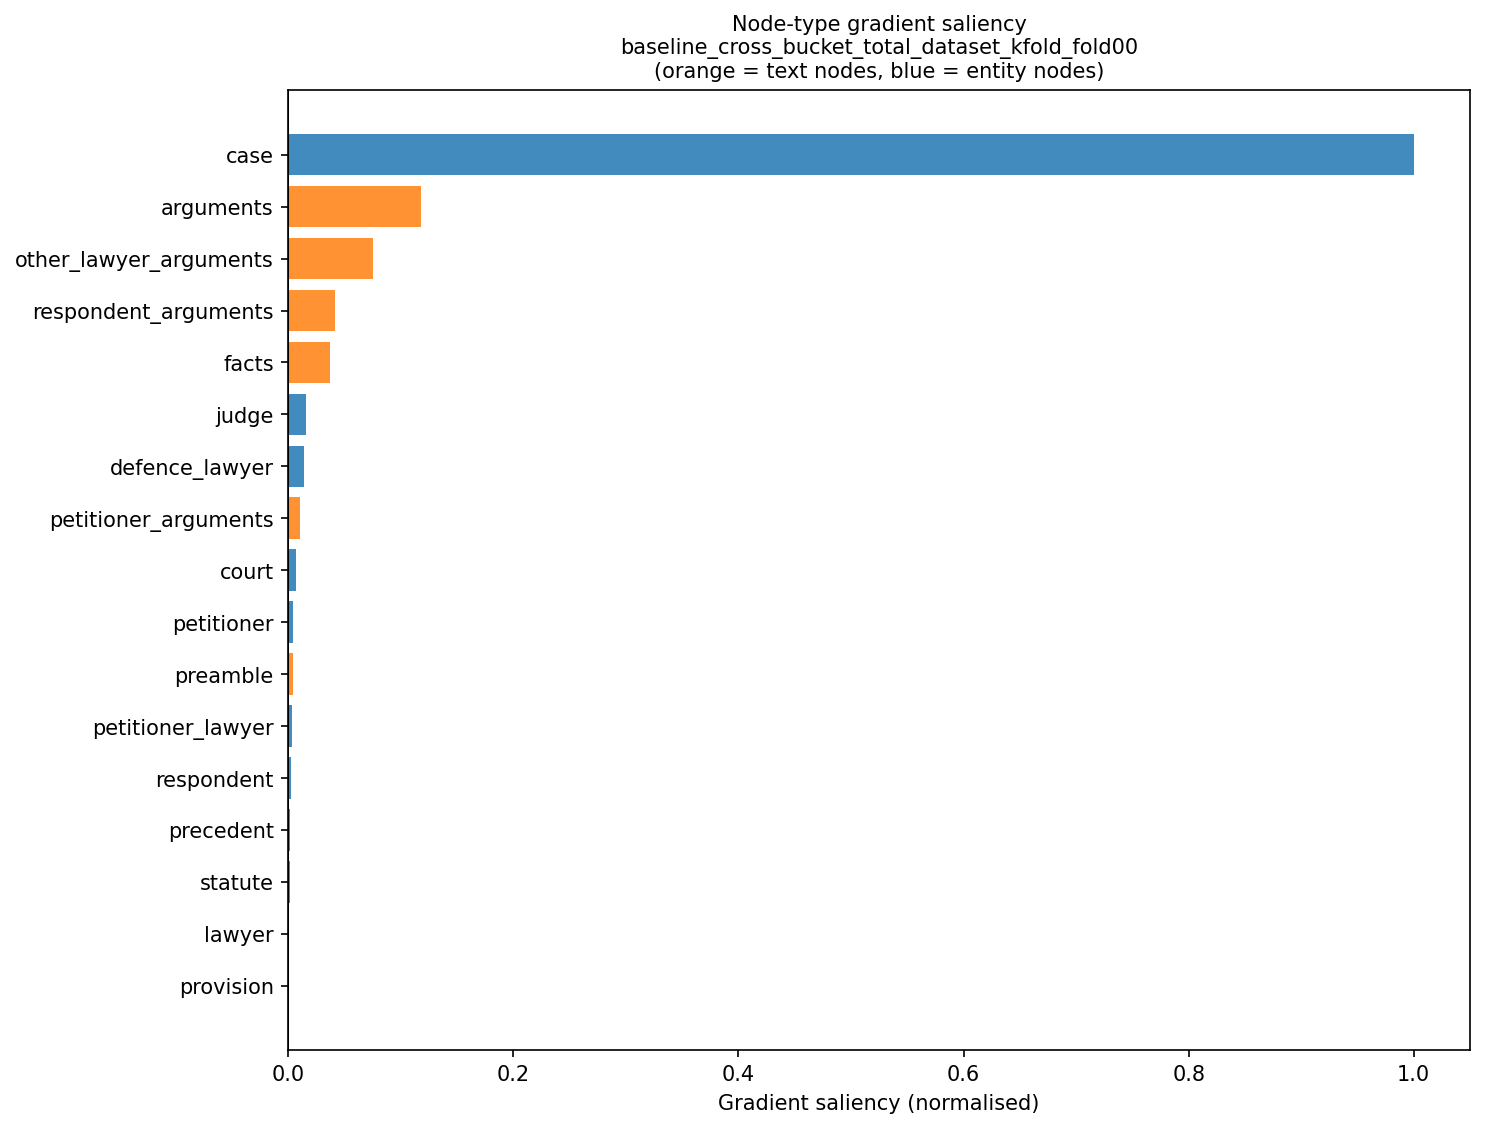
\includegraphics[width=\linewidth]{figures/baseline_cross_bucket_total_dataset_kfold_fold00_gradient_saliency.png}
  \end{minipage}\hfill
  \begin{minipage}{0.49\textwidth}
    {\color{blue}\footnotesize (b) Baseline learned relation prior heatmap\par}
    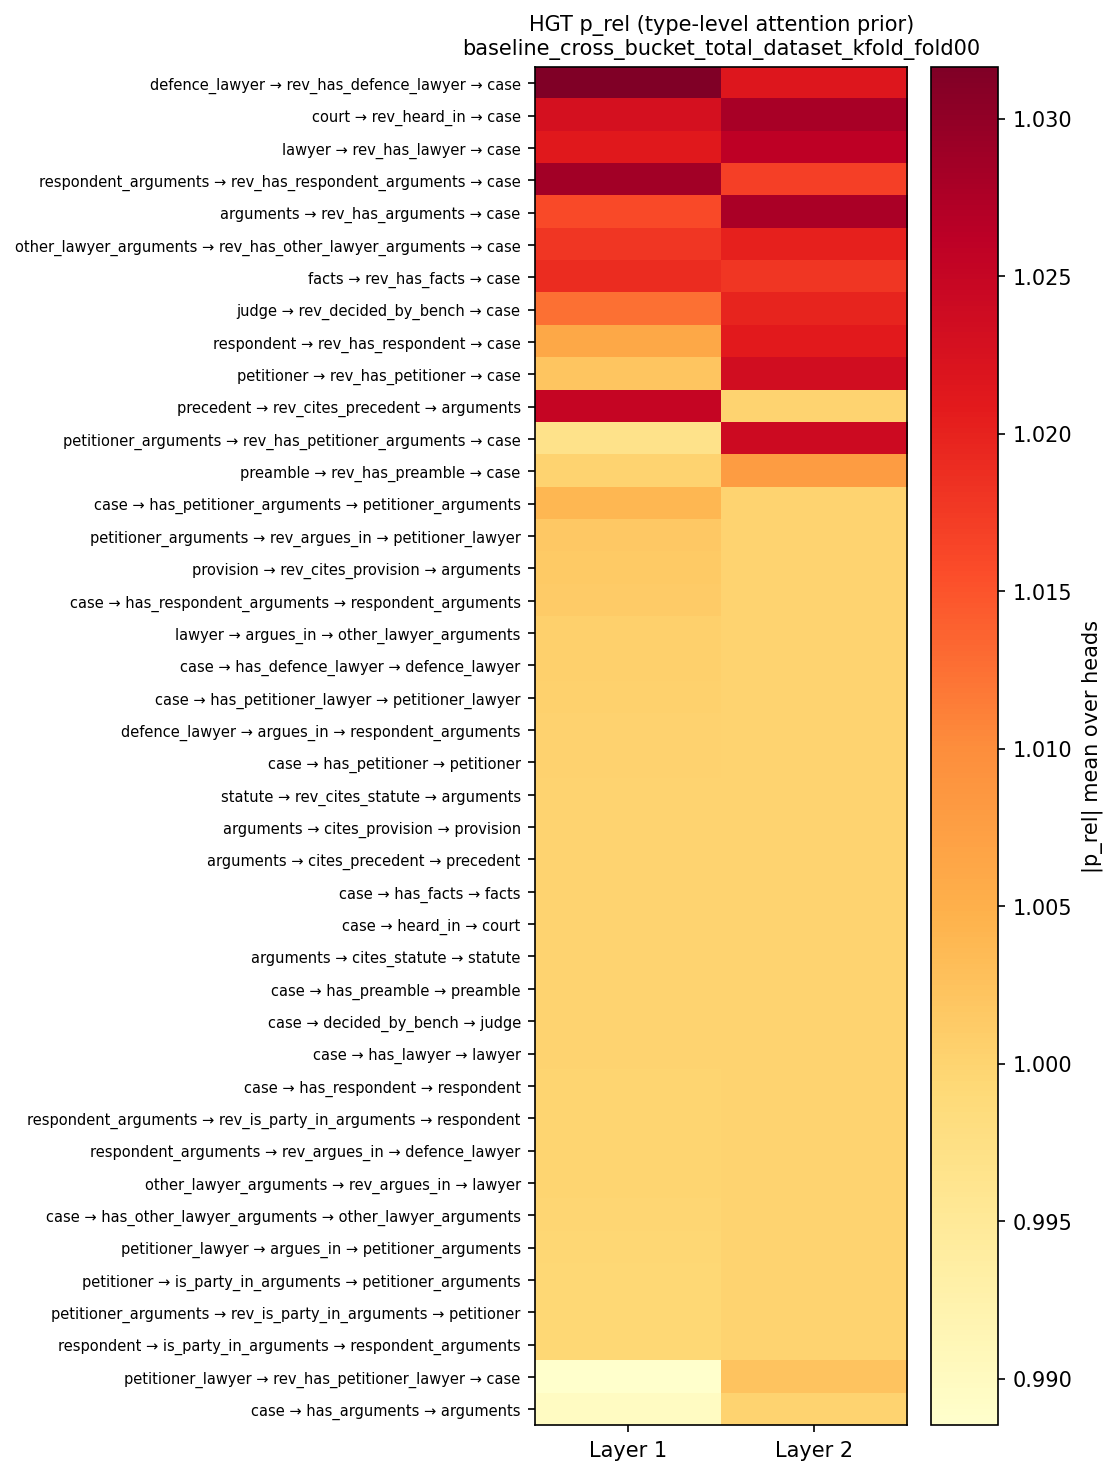
\includegraphics[width=\linewidth]{figures/baseline_cross_bucket_total_dataset_kfold_fold00_prel_heatmap.png}
  \end{minipage}
  \caption{{\color{blue}Interpretability plots for the baseline
  cross-bucket model on fold~0. The left panel visualises which node
  types contribute most to the case logit under gradient saliency; the
  right panel visualises the learned per-relation attention prior.}}
  \label{fig:attention_saliency_baseline}
\end{figure}

{\color{blue}Figure~\ref{fig:attention_saliency_baseline} makes the
interpretability claims visual. The model is overwhelmingly driven by
the case representation and the argument-bearing text nodes, not by a
single authority type. At the same time, the relation-prior heatmap
shows that the strongest learned edge types are reverse edges flowing
back into the \textsc{Case} node from text and contextual nodes. That
combination helps explain two earlier findings at once: why
\texttt{text\_only} remains surprisingly strong, and why stripping
names leaves performance almost unchanged. The model's main computation
is structured aggregation of textual legal context into the case node,
not retrieval of identity cues.\par}

\section{SHAP Feature Importance}

Because the post-GNN case embedding is only $64$-dimensional and the
downstream classifier is a logistic regression, a SHAP-style
attribution reduces to the absolute coefficient of each latent
dimension. The top dimensions on the baseline model
(\texttt{dim~16, 38, 13, 25, 29, 14, 0, 10, 27, 4}) each carry
$|\beta|\!\ge\!0.14$; the remaining $54$ dimensions contribute smaller,
more distributed weight. No single dimension dominates, which is
evidence that the case embedding is distributed rather than
collapsing onto a small set of predictive features.

\section{Embedding Visualisation (t-SNE)}

t-SNE projections of the pre-GNN and post-GNN case embeddings, coloured
by bucket (\texttt{tsne\_*\_by\_domain.png}) and by outcome label
(\texttt{tsne\_*\_by\_label.png}), complete the picture. Three
patterns appear:

\begin{enumerate}
  \item Pre-GNN embeddings cluster strongly by \emph{bucket}: the
    \texttt{bge-m3} representation of the concatenated text already
    separates the five legal domains. Label separability is weak at
    this stage.
  \item Post-GNN embeddings retain the bucket clusters but, within
    each cluster, label-colour separation is visibly improved. The
    HGT's contribution is therefore primarily \emph{within-domain}
    label structure, not between-domain re-organisation.
  \item The \texttt{no\_names} model's t-SNE is qualitatively
    indistinguishable from the baseline's, consistent with the
    probing result and the ablation result: identity information is
    not what the model is using to form the embedding.
\end{enumerate}

\begin{figure}[H]
  \centering
  \begin{minipage}{0.49\textwidth}
    {\color{blue}\footnotesize (a) Baseline pre-GNN, coloured by domain\par}
    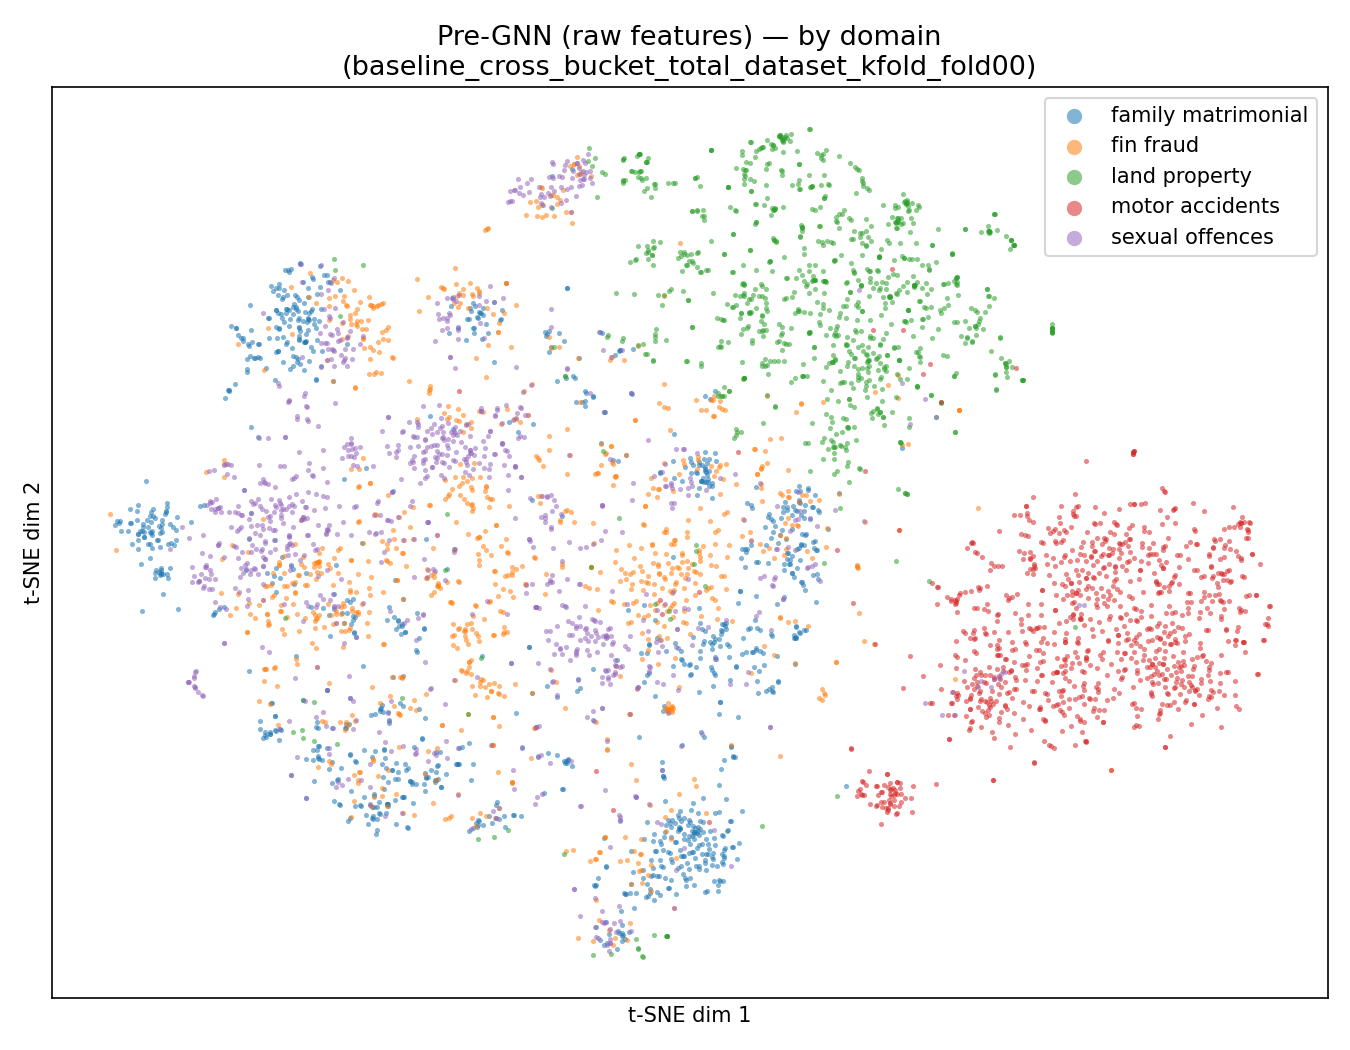
\includegraphics[width=\linewidth]{figures/baseline_cross_bucket_total_dataset_kfold_fold00_tsne_pre_by_domain.png}
  \end{minipage}\hfill
  \begin{minipage}{0.49\textwidth}
    {\color{blue}\footnotesize (b) Baseline post-GNN, coloured by domain\par}
    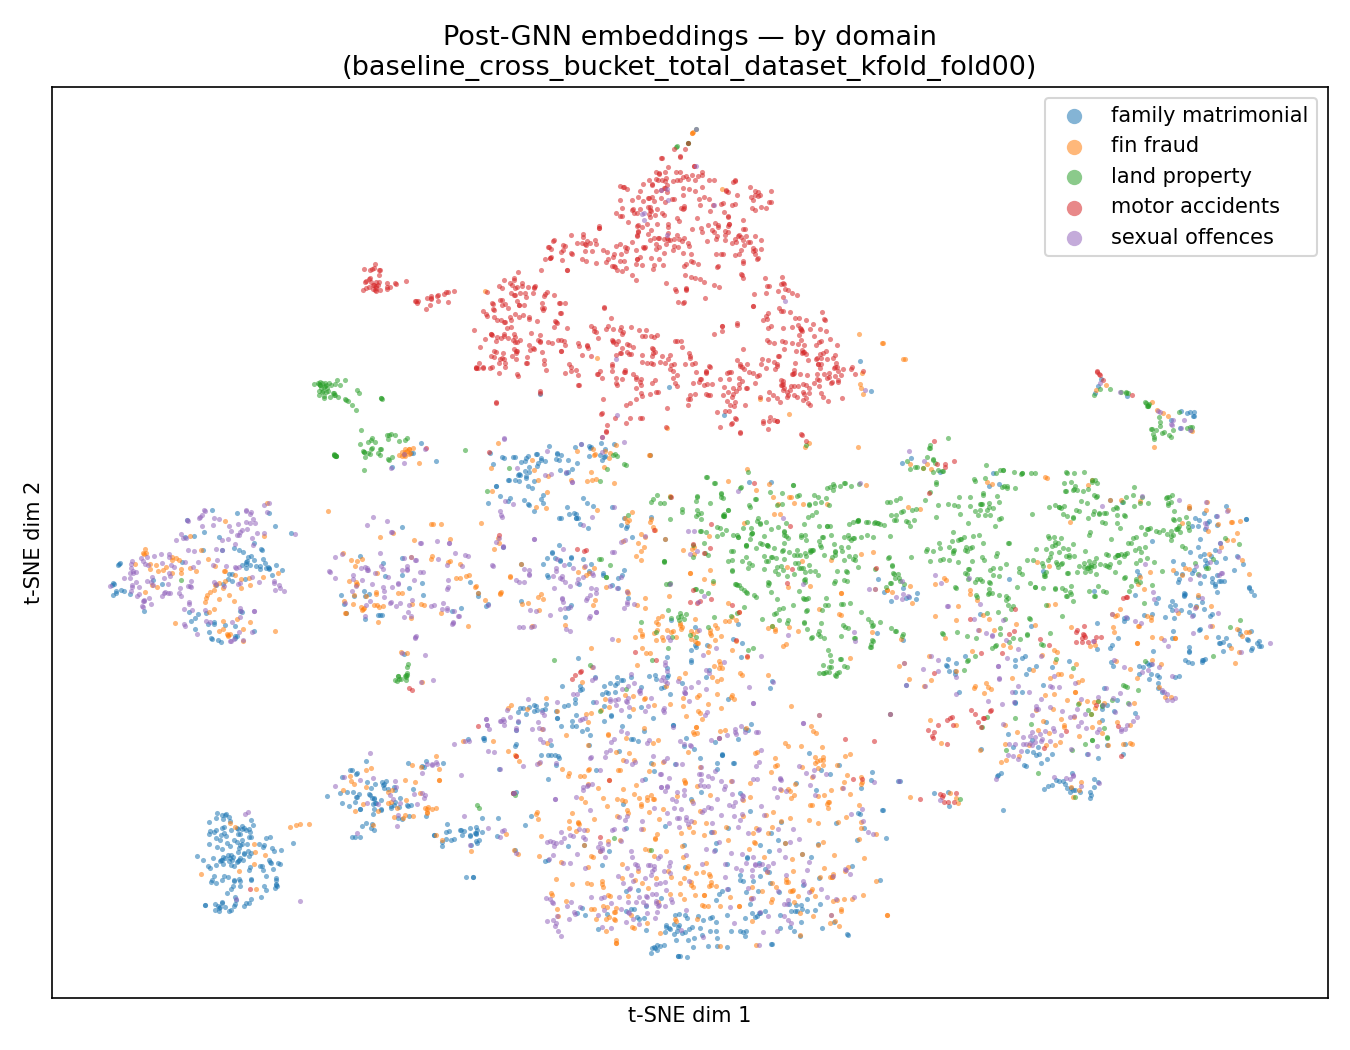
\includegraphics[width=\linewidth]{figures/baseline_cross_bucket_total_dataset_kfold_fold00_tsne_post_by_domain.png}
  \end{minipage}

  \vspace{0.5em}

  \begin{minipage}{0.49\textwidth}
    {\color{blue}\footnotesize (c) Baseline pre-GNN, coloured by label\par}
    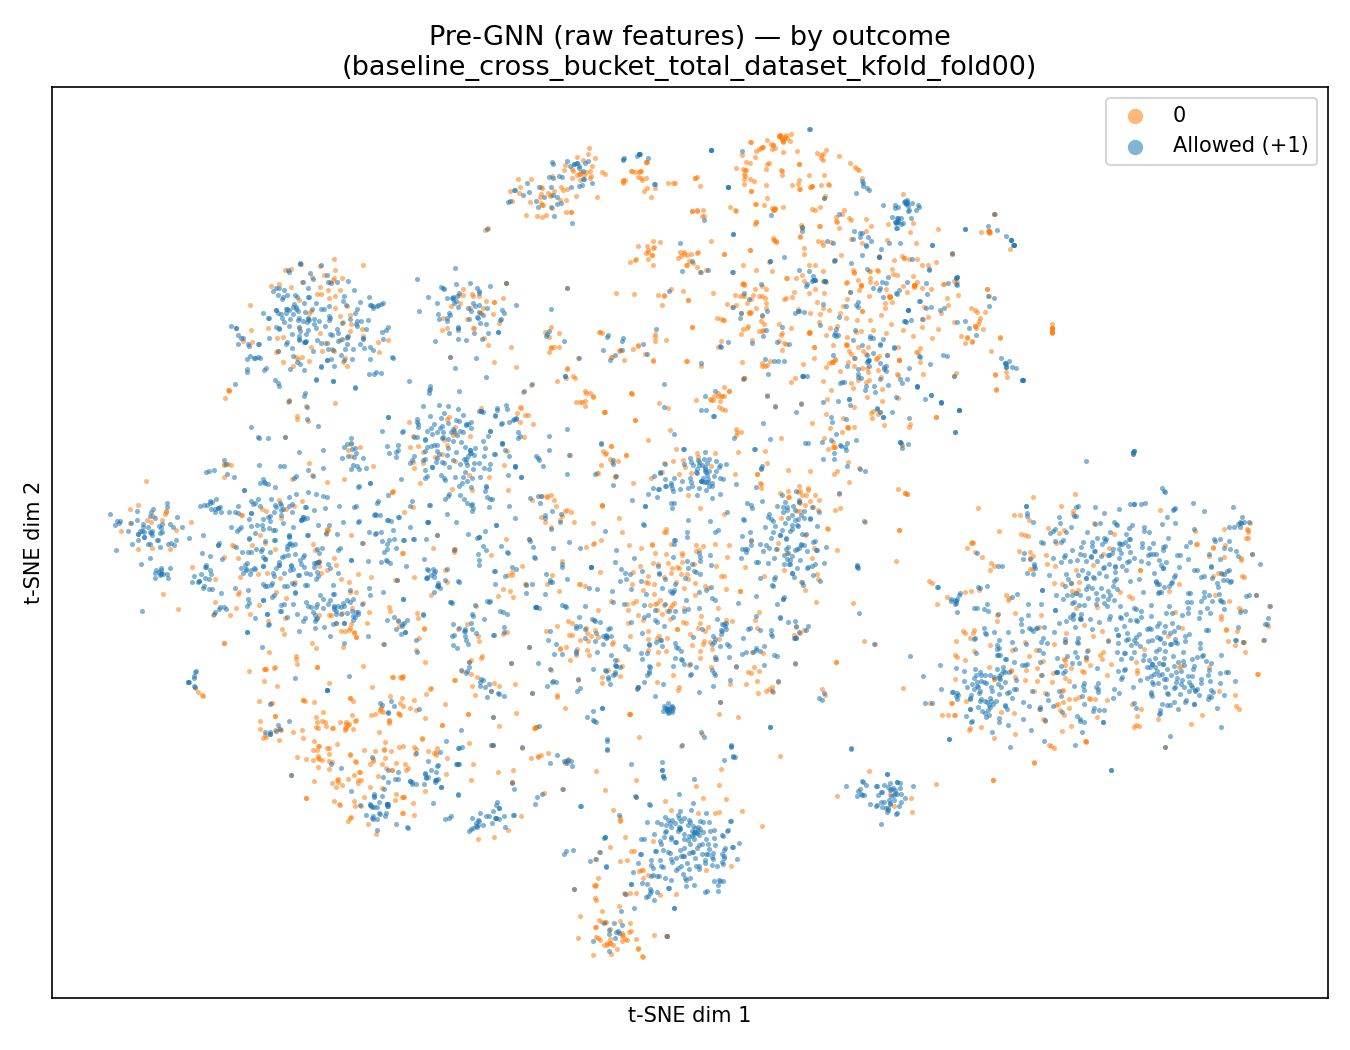
\includegraphics[width=\linewidth]{figures/baseline_cross_bucket_total_dataset_kfold_fold00_tsne_pre_by_label.png}
  \end{minipage}\hfill
  \begin{minipage}{0.49\textwidth}
    {\color{blue}\footnotesize (d) Baseline post-GNN, coloured by label\par}
    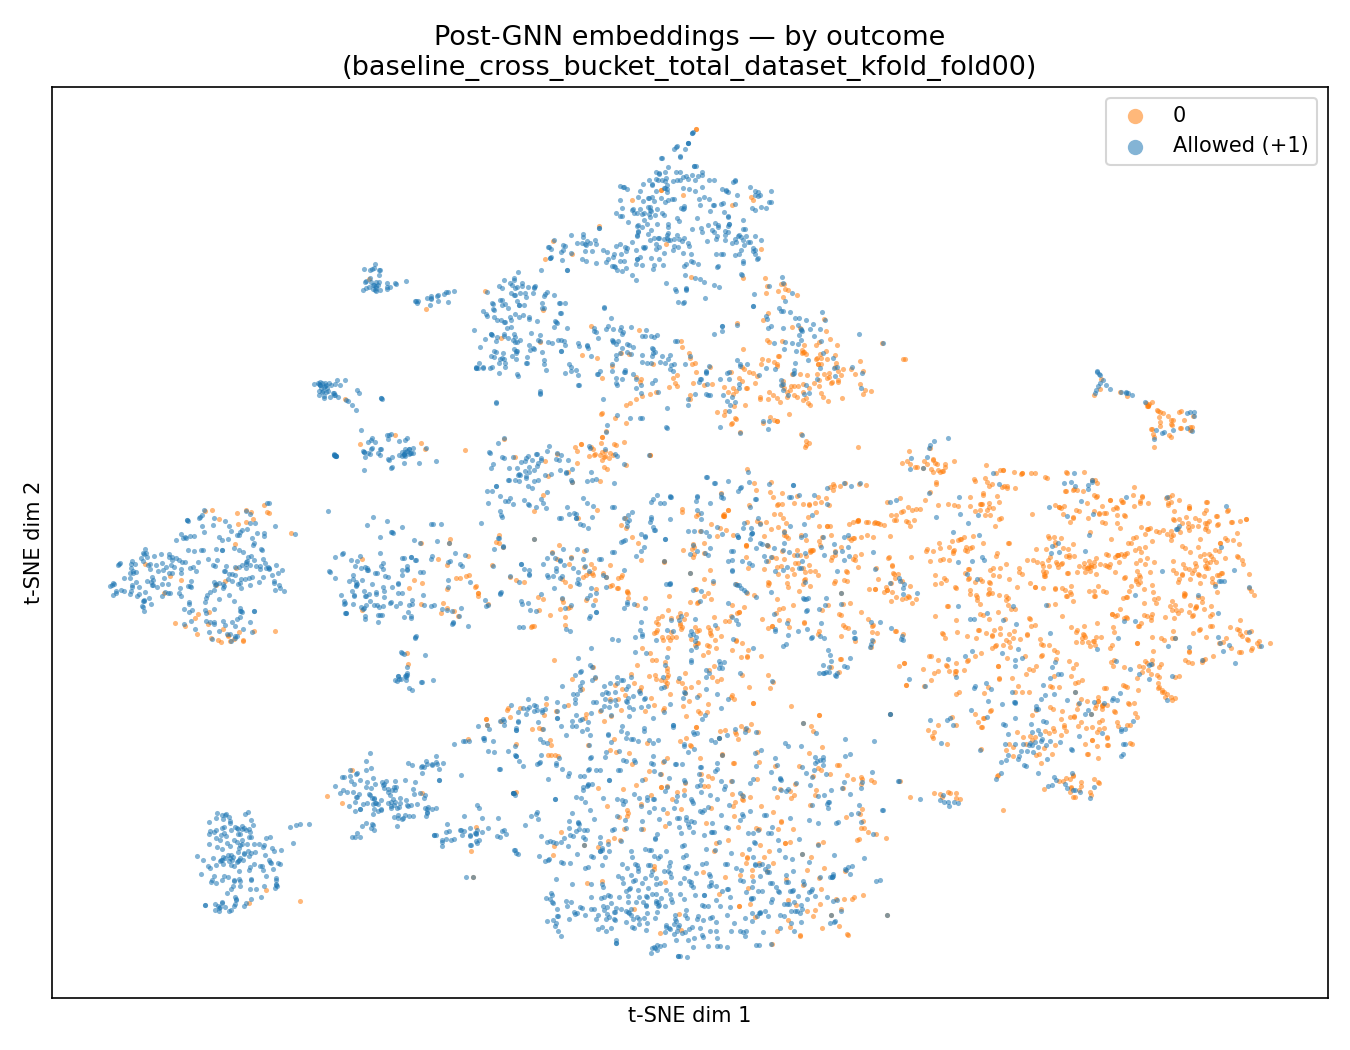
\includegraphics[width=\linewidth]{figures/baseline_cross_bucket_total_dataset_kfold_fold00_tsne_post_by_label.png}
  \end{minipage}
  \caption{{\color{blue}Baseline fold-0 t-SNE projections before and
  after graph message passing. The top row tracks domain structure; the
  bottom row tracks outcome structure.}}
  \label{fig:baseline_tsne}
\end{figure}

{\color{blue}Figure~\ref{fig:baseline_tsne} makes the geometry of the
embedding transition easier to read than the summary bullets alone.
Before graph propagation, the representation is already domain-aware:
motor-accidents and land-property form visibly coherent clusters, while
family, fraud, and sexual-offences overlap more heavily. After graph
propagation, these domain regions are preserved, but the label-coloured
view becomes more structured inside them, especially in the larger
motor-accident and land-property regions. This is visually consistent
with the probing result: the GNN is not erasing domain information, but
reorganising each domain locally in a more outcome-informative
way.\par}

\begin{figure}[H]
  \centering
  \begin{minipage}{0.49\textwidth}
    {\color{blue}\footnotesize (a) \texttt{no\_names} pre-GNN, coloured by domain\par}
    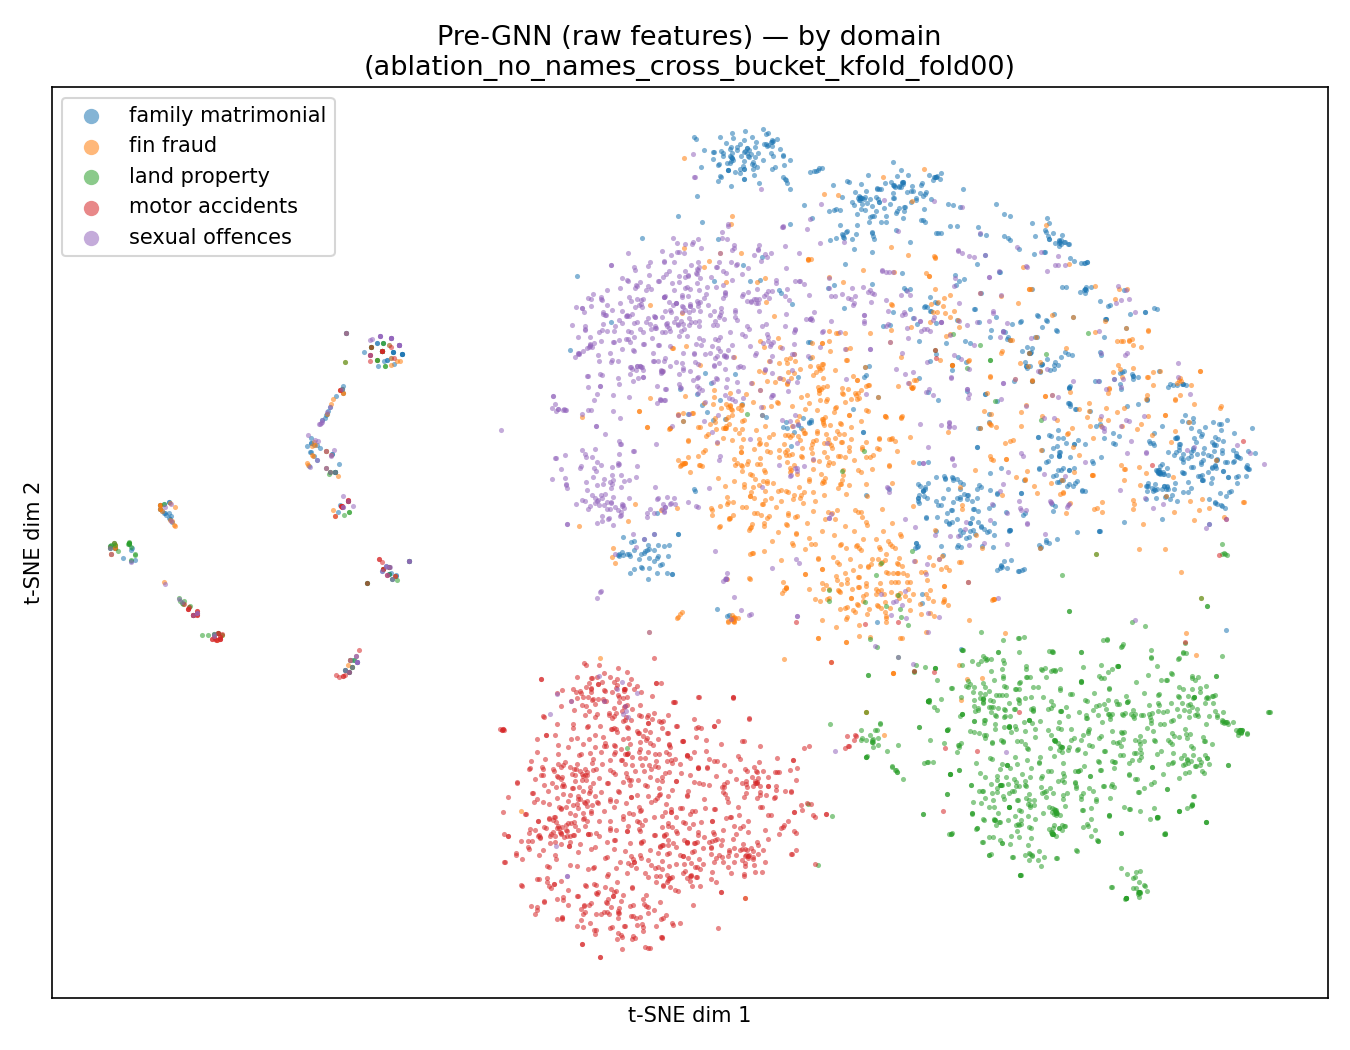
\includegraphics[width=\linewidth]{figures/ablation_no_names_cross_bucket_kfold_fold00_tsne_pre_by_domain.png}
  \end{minipage}\hfill
  \begin{minipage}{0.49\textwidth}
    {\color{blue}\footnotesize (b) \texttt{no\_names} post-GNN, coloured by domain\par}
    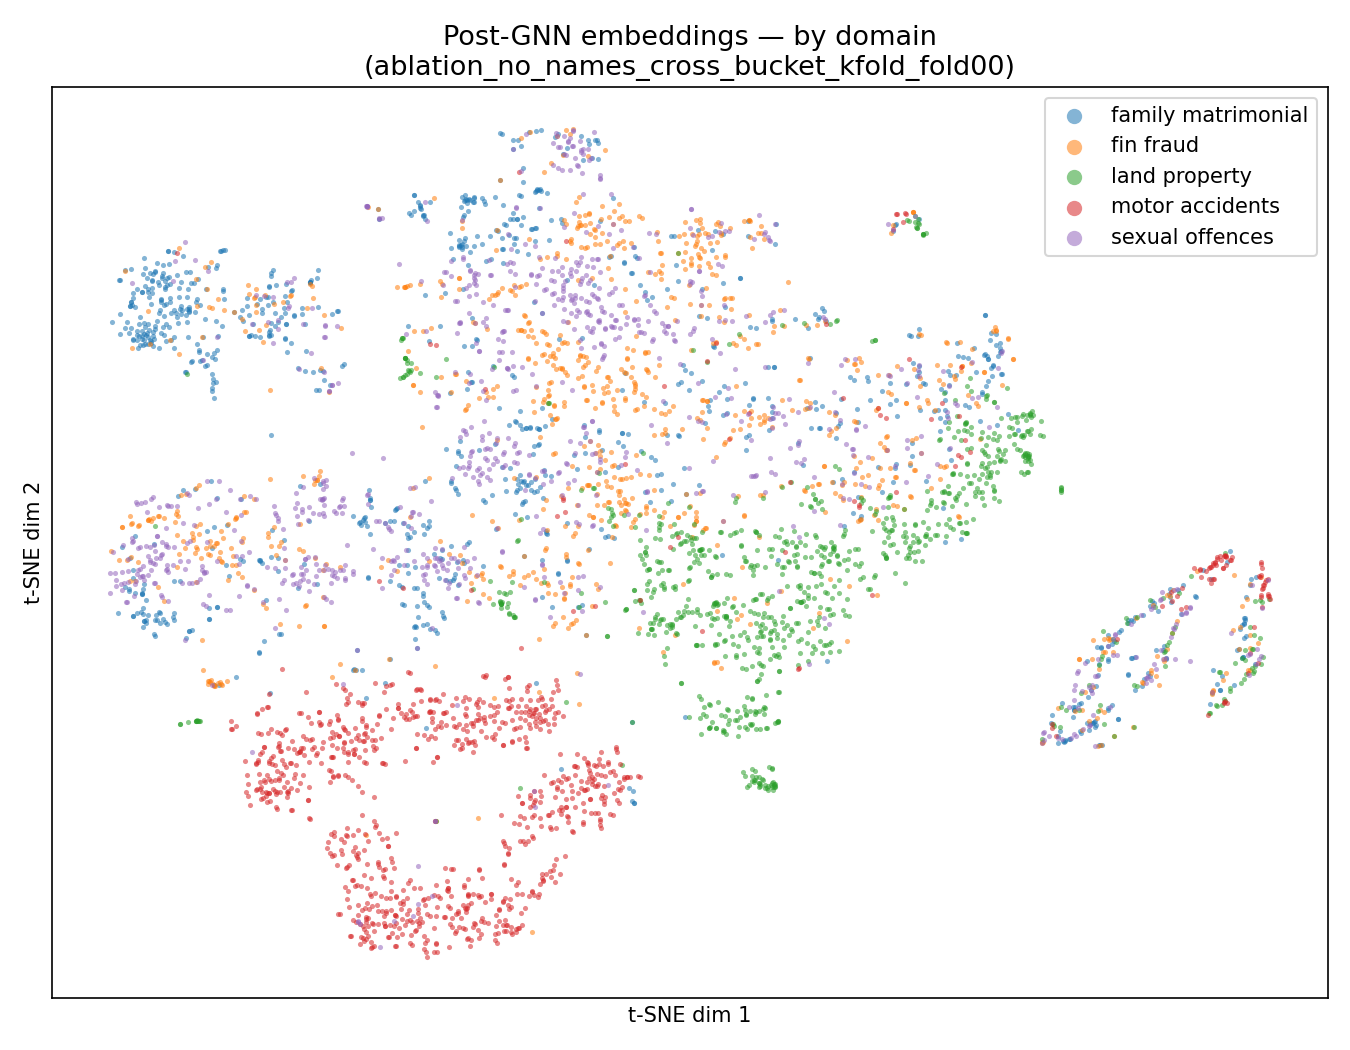
\includegraphics[width=\linewidth]{figures/ablation_no_names_cross_bucket_kfold_fold00_tsne_post_by_domain.png}
  \end{minipage}

  \vspace{0.5em}

  \begin{minipage}{0.49\textwidth}
    {\color{blue}\footnotesize (c) \texttt{no\_names} pre-GNN, coloured by label\par}
    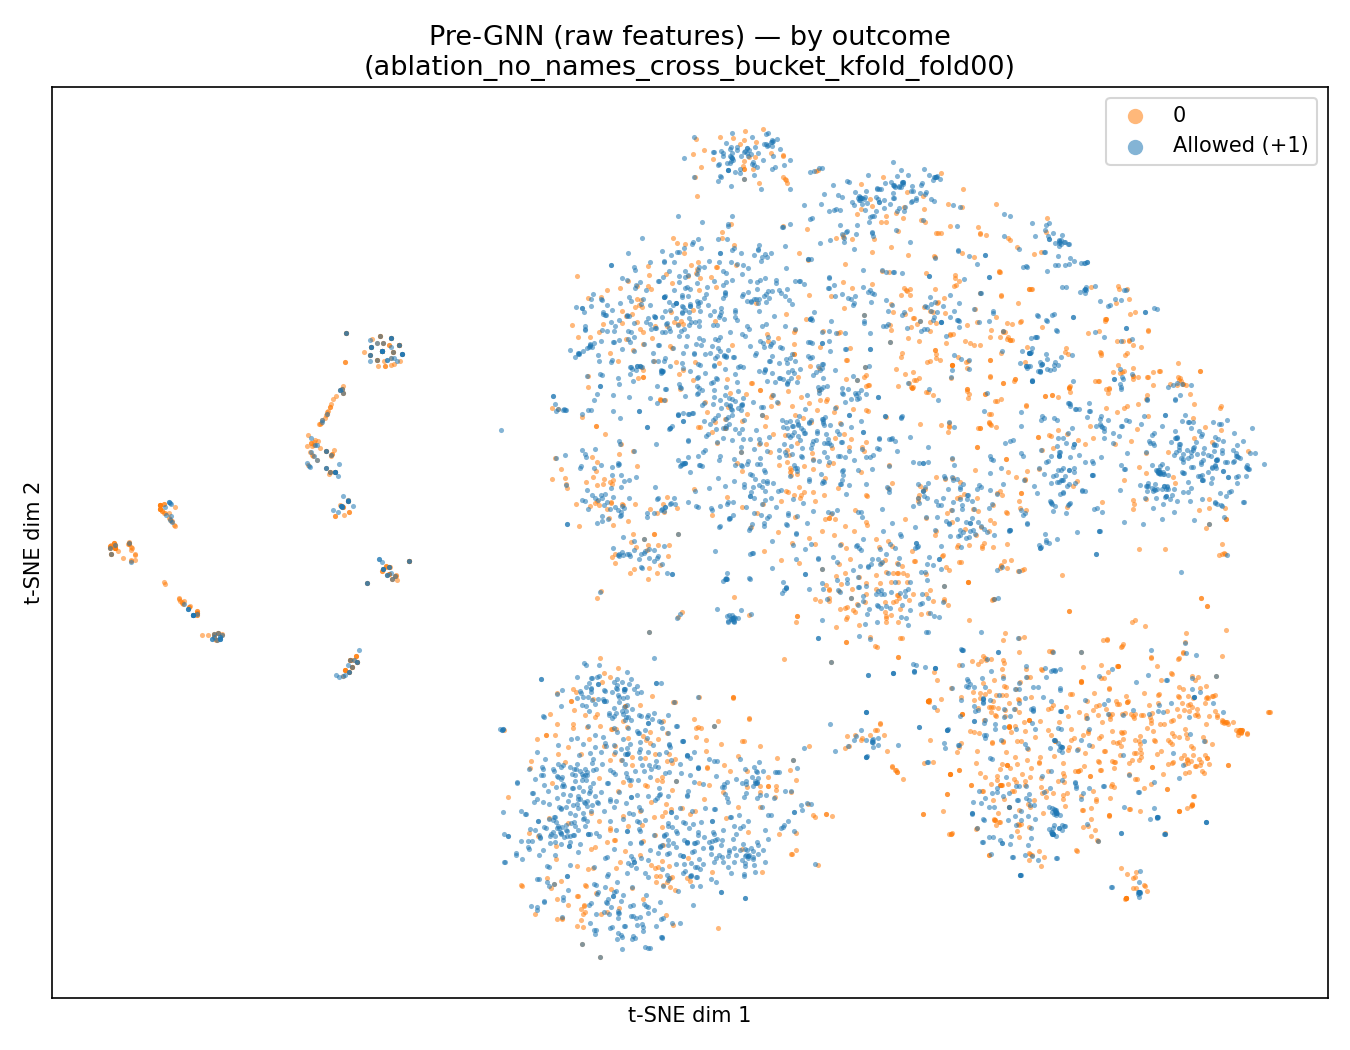
\includegraphics[width=\linewidth]{figures/ablation_no_names_cross_bucket_kfold_fold00_tsne_pre_by_label.png}
  \end{minipage}\hfill
  \begin{minipage}{0.49\textwidth}
    {\color{blue}\footnotesize (d) \texttt{no\_names} post-GNN, coloured by label\par}
    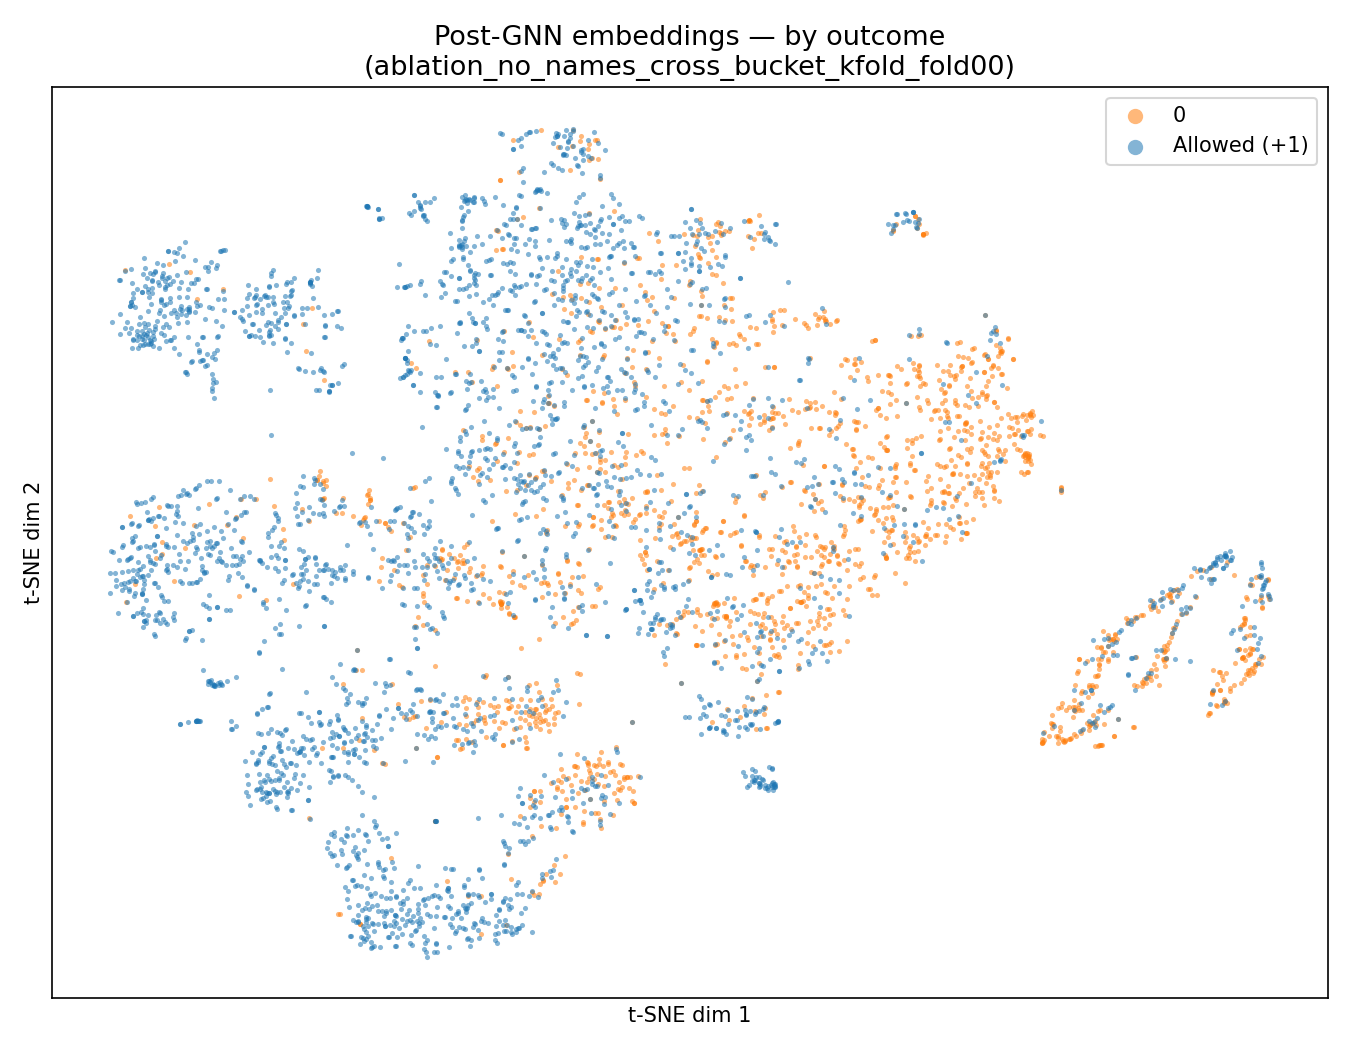
\includegraphics[width=\linewidth]{figures/ablation_no_names_cross_bucket_kfold_fold00_tsne_post_by_label.png}
  \end{minipage}
  \caption{{\color{blue}Corresponding fold-0 t-SNE projections for the
  \texttt{no\_names} ablation.}}
  \label{fig:no_names_tsne}
\end{figure}

{\color{blue}The \texttt{no\_names} t-SNEs in
Figure~\ref{fig:no_names_tsne} reinforce the ablation result from a
different angle. Removing names changes the exact geometry of the
projection, but it does not collapse the domain structure and it does
not remove the post-GNN improvement in label organisation. In other
words, the model still finds a structured outcome space after graph
propagation even when party, lawyer, and judge names are withheld. The
visual similarity is not exact -- t-SNE should not be over-read at that
level -- but the qualitative conclusion is the same as in the accuracy
tables: identity cues are not the dominant organising principle of the
learned case embedding.\par}

\section{Error Analysis}

\noindent\textbf{Error analysis across ablations.} The baseline's
per-domain error pattern -- family-matrimonial $0.802$, fin-fraud
$0.754$, land-property $0.778$, motor-accidents $0.821$,
sexual-offences $0.777$ -- is nearly identical to the
\texttt{no\_names} model's ($0.797, 0.750, 0.782, 0.807, 0.770$),
reinforcing that the two variants share a prediction policy up to
small, within-noise differences. The common pattern across every
ablation -- motor-accidents easiest, sexual-offences hardest -- is a
property of the data, not of the model.

\begin{figure}[H]
  \centering
  \begin{minipage}{0.49\textwidth}
    {\color{blue}\footnotesize (a) Baseline accuracy by statute-count bucket\par}
    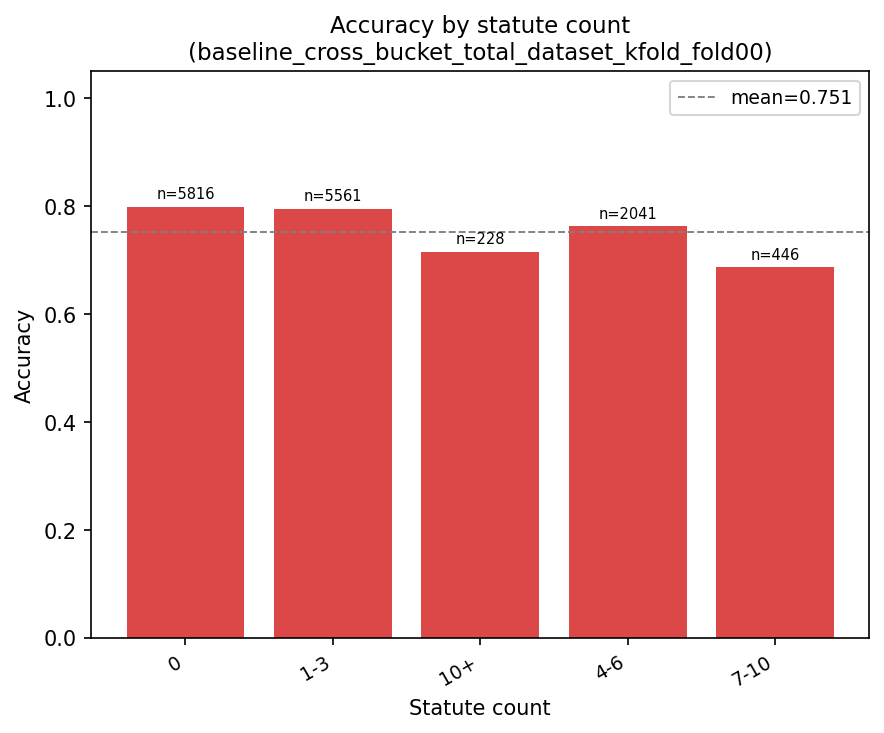
\includegraphics[width=\linewidth]{figures/baseline_cross_bucket_total_dataset_kfold_fold00_error_by_statute.png}
  \end{minipage}\hfill
  \begin{minipage}{0.49\textwidth}
    {\color{blue}\footnotesize (b) \texttt{no\_names} accuracy by statute-count bucket\par}
    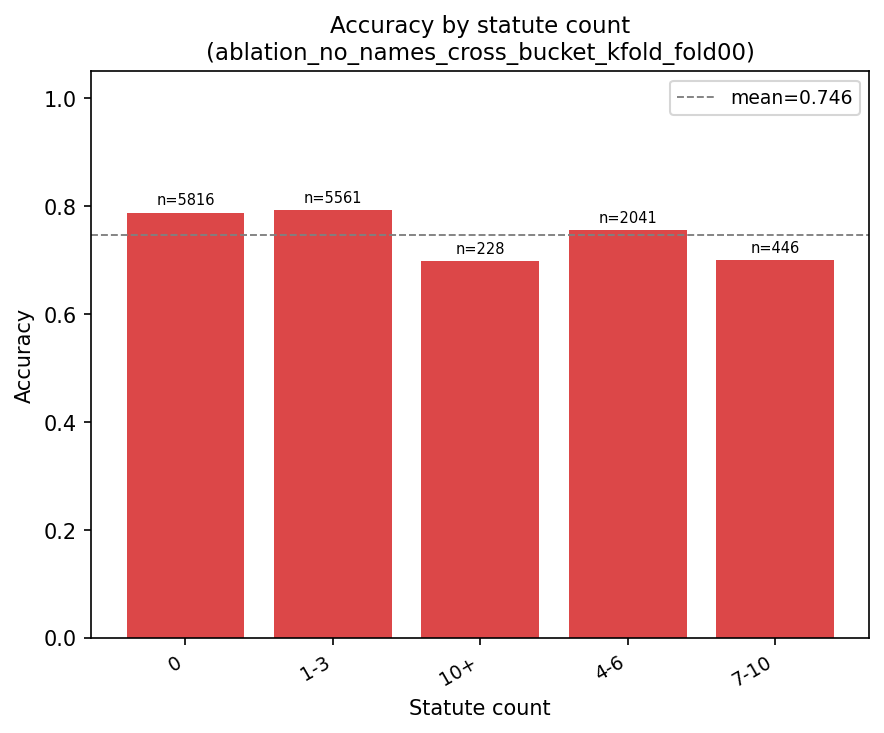
\includegraphics[width=\linewidth]{figures/ablation_no_names_cross_bucket_kfold_fold00_error_by_statute.png}
  \end{minipage}
  \caption{{\color{blue}Held-out fold-0 accuracy as a function of the
  number of statute nodes attached to a case, for the baseline and
  \texttt{no\_names} models.}}
  \label{fig:error_by_statute_count}
\end{figure}

{\color{blue}Figure~\ref{fig:error_by_statute_count} adds an error
pattern that is not visible in the domain-level accuracy tables.
Accuracy is highest when a case cites few statutes and falls once the
authority neighbourhood becomes dense: in the baseline, cases with 0 or
1--3 statute nodes sit near $0.80$ accuracy, while the 7--10 and 10+
buckets are closer to $0.69$--$0.71$. The \texttt{no\_names} model
shows essentially the same curve. This suggests that many of the
residual errors are concentrated in doctrinally crowded cases rather
than in identity-sensitive ones. That is an important distinction: the
hard cases are not those where the model lacks names, but those where
several statutory frames and remedial pathways coexist in the same
judgment.\par}

\begin{figure}[H]
  \centering
  \begin{minipage}{0.49\textwidth}
    {\color{blue}\footnotesize (a) Baseline accuracy by facts-length bucket\par}
    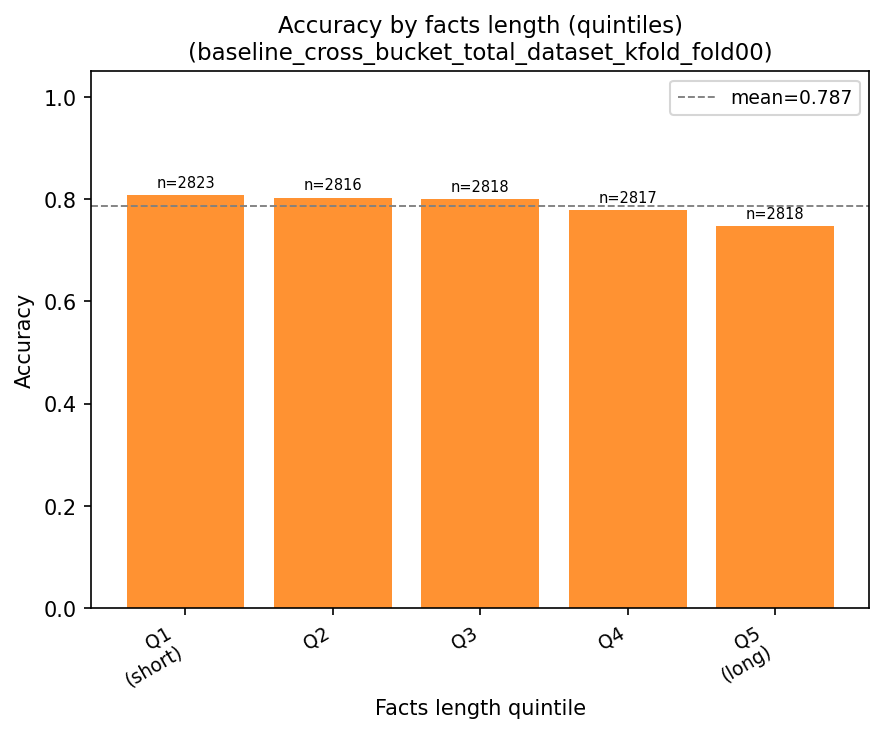
\includegraphics[width=\linewidth]{figures/baseline_cross_bucket_total_dataset_kfold_fold00_error_by_facts_len.png}
  \end{minipage}\hfill
  \begin{minipage}{0.49\textwidth}
    {\color{blue}\footnotesize (b) \texttt{no\_names} accuracy by facts-length bucket\par}
    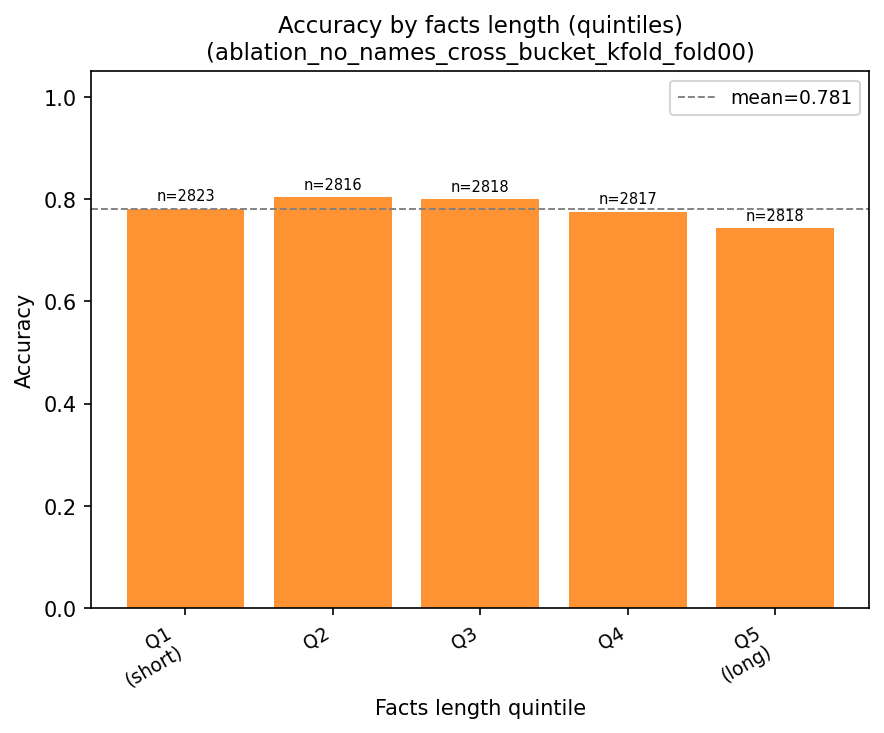
\includegraphics[width=\linewidth]{figures/ablation_no_names_cross_bucket_kfold_fold00_error_by_facts_len.png}
  \end{minipage}
  \caption{{\color{blue}Held-out fold-0 accuracy as a function of the
  length of the facts section, grouped into quintiles from shortest to
  longest, for the baseline and \texttt{no\_names} models.}}
  \label{fig:error_by_facts_length}
\end{figure}

{\color{blue}Figure~\ref{fig:error_by_facts_length} is useful for a
different reason than Figure~\ref{fig:error_by_statute_count}: it tests
whether the remaining errors are concentrated in structurally long
judgments. They are. In the baseline, accuracy falls from about $0.81$
on the shortest-facts quintile to about $0.75$ on the longest-facts
quintile; the \texttt{no\_names} model shows nearly the same decline.
This matters because it links the error analysis back to the ablation
story. The modest, domain-specific gains from
\texttt{hierarchical\_enc} are easier to interpret once the failure
pattern is visible: longer factual narratives do create a harder
representation problem, but the difficulty comes from document
complexity rather than from named entities or party identity.\par}
